Le contrôleur est l'élément central du réseau SDN, puisqu'il offre au niveau de son interface nord, une API pour développer des applications réseau, et, au niveau de son interface sud, il contrôle les entités réseaux se chargeant du plan de données, avec le protocole OpenFlow.

Pour fonctionner correctement, le contrôleur doit avoir la représentation interne la plus exacte possible du réseau qu'il manipule. OpenFlow prévoit certains paquets spécialisés (requêtes de configuration, auxquelles les switchs répondent en renseignant leur état). Mais ce n'est pas suffisant, puisque les switchs eux-mêmes ne sont pas capables de renseigner le contrôleur sur la topologie alentours. C'est pourquoi certains mécanismes sont mis en place (qui dépendent généralement du contrôleur, même si, devant utiliser des protocoles classiques compréhensibles par des switchs, les possibilités restent limitées).\\
Le mécanisme que j'ai été amené à constater est celui de l'utilisation de paquets LLDP fabriqués par le contrôleur et envoyés aux switchs sous forme de PACKET\_OUT (voir note en base de page à la page 15 pour la définition, et utiliser la figure à la page suivante pour mieux comprendre le mécanisme). En recevant un tel paquet, un switch va le retransmettre en broadcast aux switchs alentours, qui, normalement, sont configurés pour le renvoyer en PACKET\_IN au contrôleur (comportement par défaut, si aucun flux gérant ce type de paquet n'est spécifié, ce qui est préférable). Or, un PACKET\_IN encapsule toutes les informations nécessaires au contrôleur pour mettre à jour la topologie locale : en vérifiant que c'est bien lui qui est à l'origine de l'émission du paquet LLDP initial (avec un champ spécial par exemple), il sait que le switch émetteur du PACKET\_IN est relié au switch auquel il avait précédemment envoyé un PACKET\_OUT, ces premiers étant des encapsulations de paquets réels circulant sur le réseau, on peut donc y lire des adresses Ethernet, des adresses IP, .... La question de la confiance relative à la réception de tels paquets est cruciale et on va voir par la suite qu'il est relativement aisé d'attaquer le contrôleur par ce biais.\\

\begin{figure}[h]
  	\centering
  	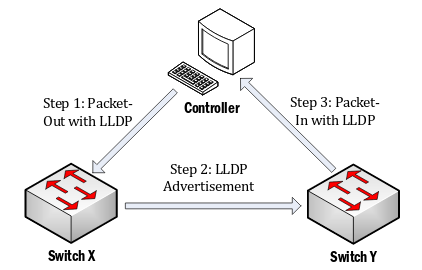
\includegraphics[width=0.6\textwidth]{lldp.png}
  	\caption{Mécanisme de découverte de topologie par envoi de paquets LLDP}
\end{figure}

Tout contrôleur doit donc disposer d'un socle logiciel permettant de communiquer avec les différentes entités du réseau ainsi que d'utiliser ce dont il dispose pour établir la topologie virtuelle la plus ressemblante à la réalité possible.

Pour permettre l'écriture d'applications directement sur le contrôleur, celui-ci doit fournir, au niveau de son interface nord, une API qui dans la mesure du possible doit permettre au développeur de considérer  le réseau comme une boîte noire (d'écrire du code sans se soucier de la façon dont le réseau se réorganisera physiquement).

Le contrôleur est alors la pièce logicielle qui lie les deux interfaces, et doit donc disposer d'un cœur logique qui traduit des intentions abstraites (par exemple, une application reçoit un paquet qu'elle reconnaît en provenance d'un certain hôte et souhaite créer une route entre cet hôte et sa destination : elle doit pouvoir le faire sans se préoccuper des messages OpenFlow que le contrôleur va envoyer pour créer la route) en instructions qui seront données aux switchs réels.

Parmi les contrôleurs SDN les plus connus, on trouve notamment NOX (premier contrôleur SDN, 2008, rendu open source depuis), POX (juin 2011, en python), OpenDayLight (avril 2013, open source, crée par The Linux Foundation), ONOS (l'objet final de ce stage, décembre 2014, open source, crée par l'Open Networking lab puis développement repris par The Linux Foundation en 2015), et bien d'autres (Beacon, RoseMary, Ryu ...). Certains projets se ressemblent énormément au niveau des choix effectués (langages utilisés, paradigmes ...). Par exemple OpenDayLight et ONOS sont deux contrôleurs très proches dans ce qu'ils offrent (Java, architecture OSGi, sécurité vue comme un élément crucial, ...).